\documentclass{beamer}
\usetheme{Boadilla}

\usepackage{graphicx}
\usepackage{subcaption}
\usepackage{csvsimple}

\newcommand*{\presentationgoldparispath}{../presentation_230120_gold2022_paris/fig/}%

% Change size of footnotes
\renewcommand{\footnotesize}{\fontsize{5pt}{5pt}\selectfont}
\title{Pleiotropic expression quantitative trait loci are located in cis-regulatory modules, closer to more target genes and with smaller effects on the genes}
\subtitle{Centuri Day 2023}
\author{Aitor Gonz\'alez}
\institute{Aix Marseille Univ, INSERM, TAGC}
\date{May 11, 2023}

% Add section slide
\AtBeginSection[]
{
\begin{frame}
\frametitle{Table of Contents}
\tableofcontents[currentsection]
\end{frame}
}

\begin{document}

%%%%%%%%%%%%%%%%%%%%%%%%%%%%%%%%%%%%%%%%%%%%%%%%%%%%%%%%%%%%%%%%%%%%%%%%%%%%%%%%
\begin{frame}

\titlepage

\end{frame}


\section{Introduction} %%%%%%%%%%%%%%%%%%%%%%%%%%%%%%%%%%%%%%%%%%%%%%%%%%%%%%%%%%%%%%

%%%%%%%%%%%%%%%%%%%%%%%%%%%%%%%%%%%%%%%%%%%%%%%%%%%%%%%%%%%%%%%%%%%%%%%%%%%%%%%%
\begin{frame}
\frametitle{Genetic variants and diseases}

\begin{itemize}
\item Phenotypic differences between human populations are mostly coded in frequent genetic variants
\item These genetic variants also cause different disease susceptibility
\item Large datasets of associations have shown that many genetic variants change simultaneously susceptibility to many diseases, ie. the variants are pleiotropic
\end{itemize}
%
\vfill
%
What is the molecular mechanism and effect of tissue of these variants?

\end{frame}

%%%%%%%%%%%%%%%%%%%%%%%%%%%%%%%%%%%%%%%%%%%%%%%%%%%%%%%%%%%%%%%%%%%%%%%%%%%%%%%%
\begin{frame}
\frametitle{Expression quantitative trait loci (eQTL)}

\begin{itemize}
\item Quantitative trait loci (QTL) are variants associated with changes of quantitative phenotypes
\item Expression (eQTL) are variants associated with changes of gene expression in a given tissue
\item eQTLs provide a putative molecular mechanism of a variant
\end{itemize}
%
\vfill
%
What are the properties of pleiotropic eQTLs?

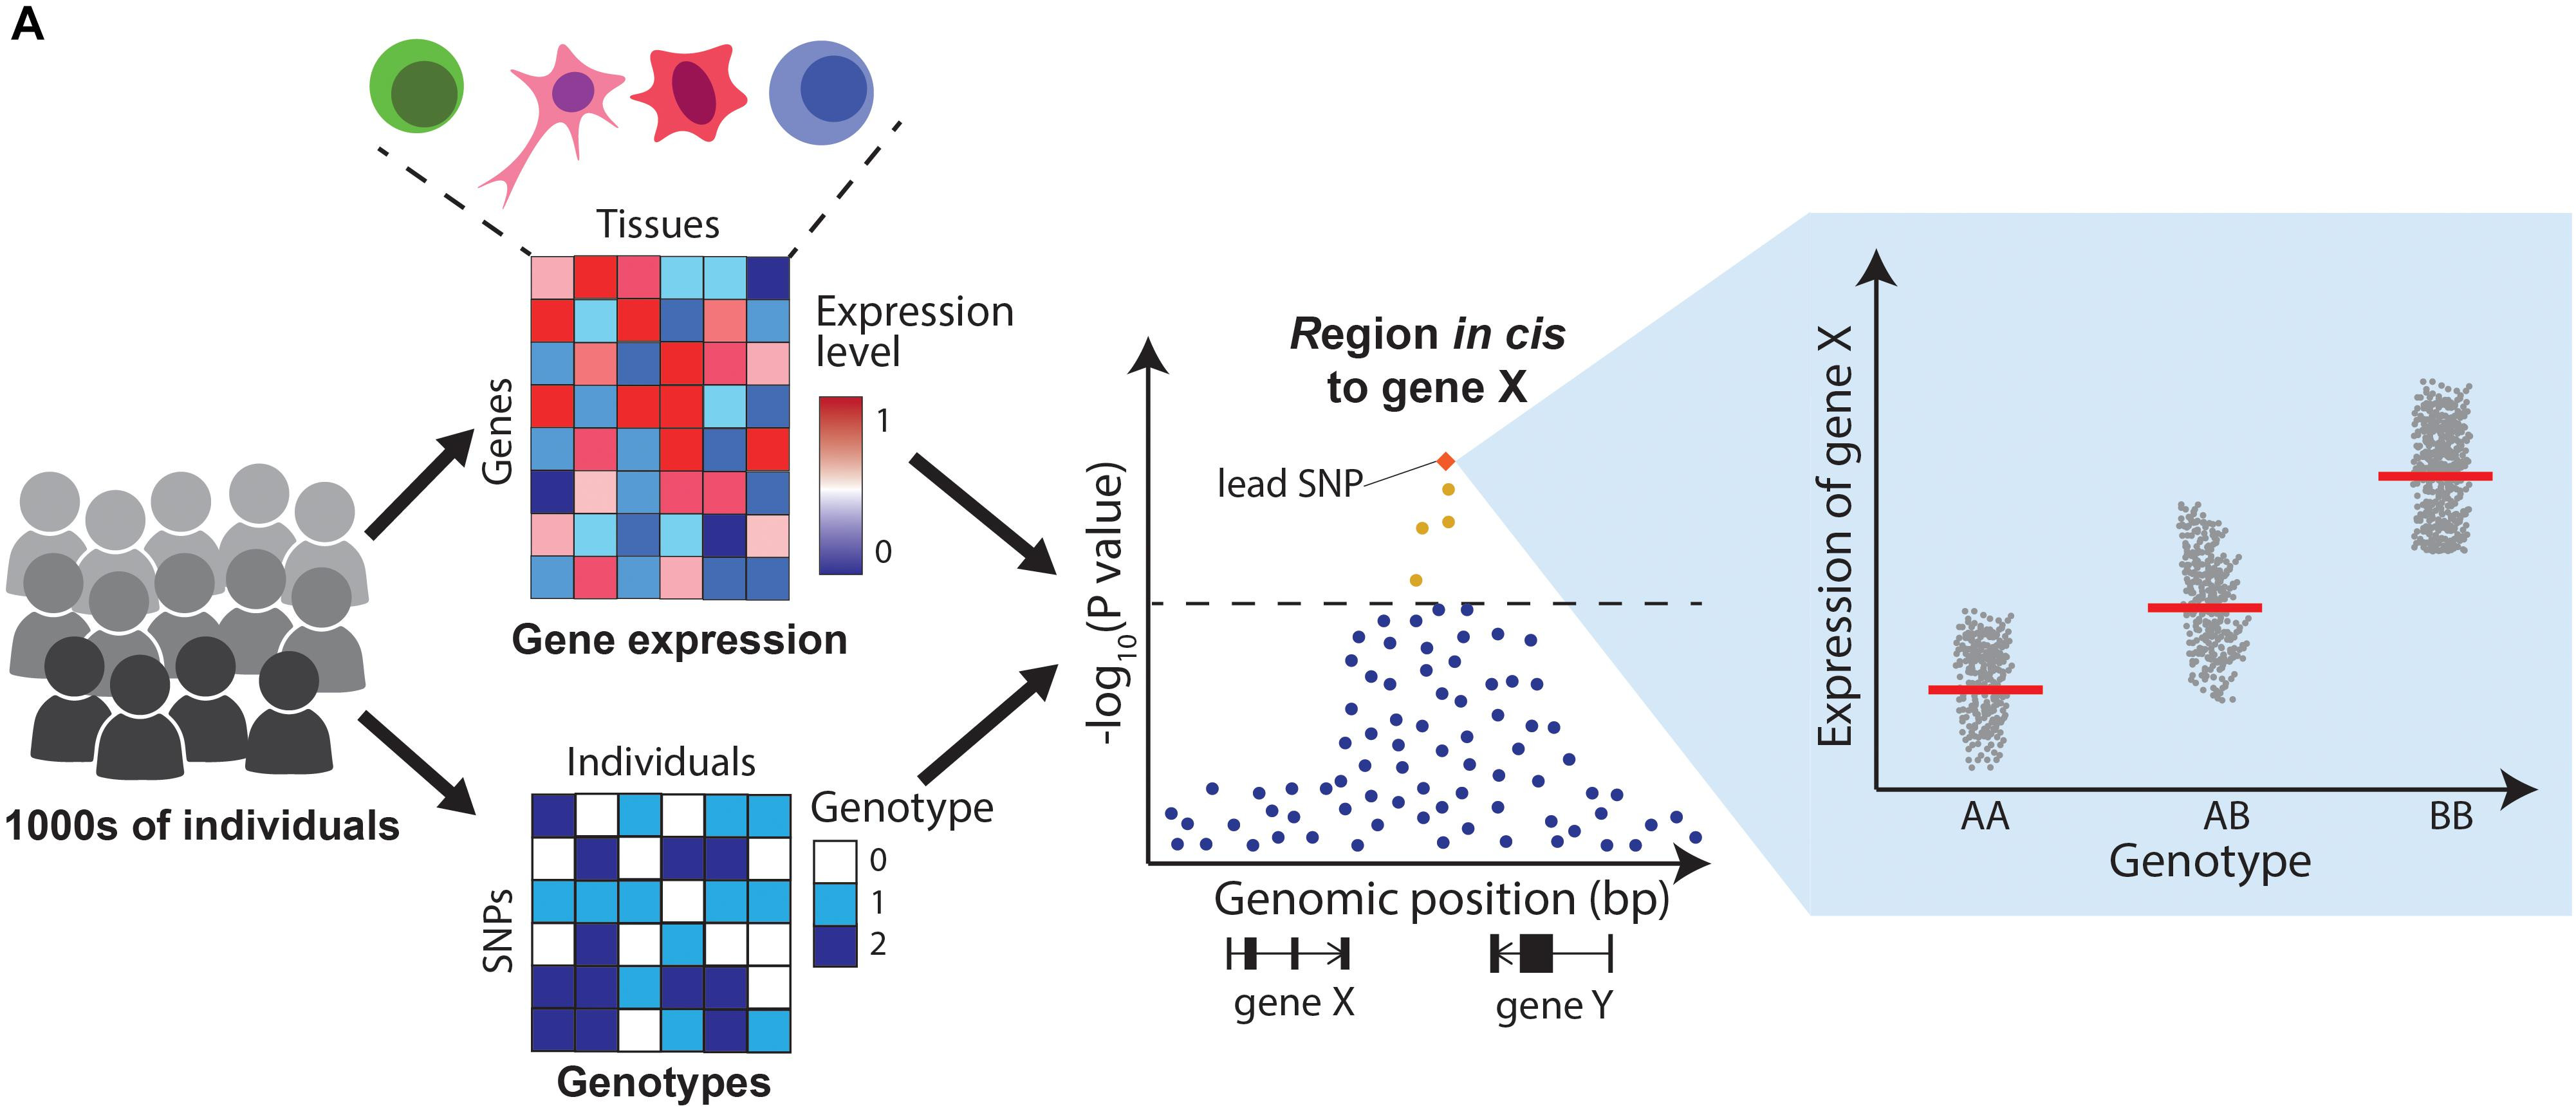
\includegraphics[width=\textwidth]{\presentationgoldparispath/doi_10.3389_fgene.2020.00424_fig4a.jpg}

\let\thefootnote\relax\footnotetext{Cano-Gamez et al. 2020. doi:10.3389/fgene.2020.00424}
\end{frame}

%%%%%%%%%%%%%%%%%%%%%%%%%%%%%%%%%%%%%%%%%%%%%%%%%%%%%%%%%%%%%%%%%%%%%%%%%%%%%%%%
\begin{frame}
\frametitle{Approach}

\begin{enumerate}
\item Compute colocalization of eQTLs and GWAS variants
\item Split eQTLs by the number of associated disease categories
\item Compare properties of pleiotropic eQTLs
\end{enumerate}
%
\vfill
%
What are the properties of pleiotropic eQTLs?

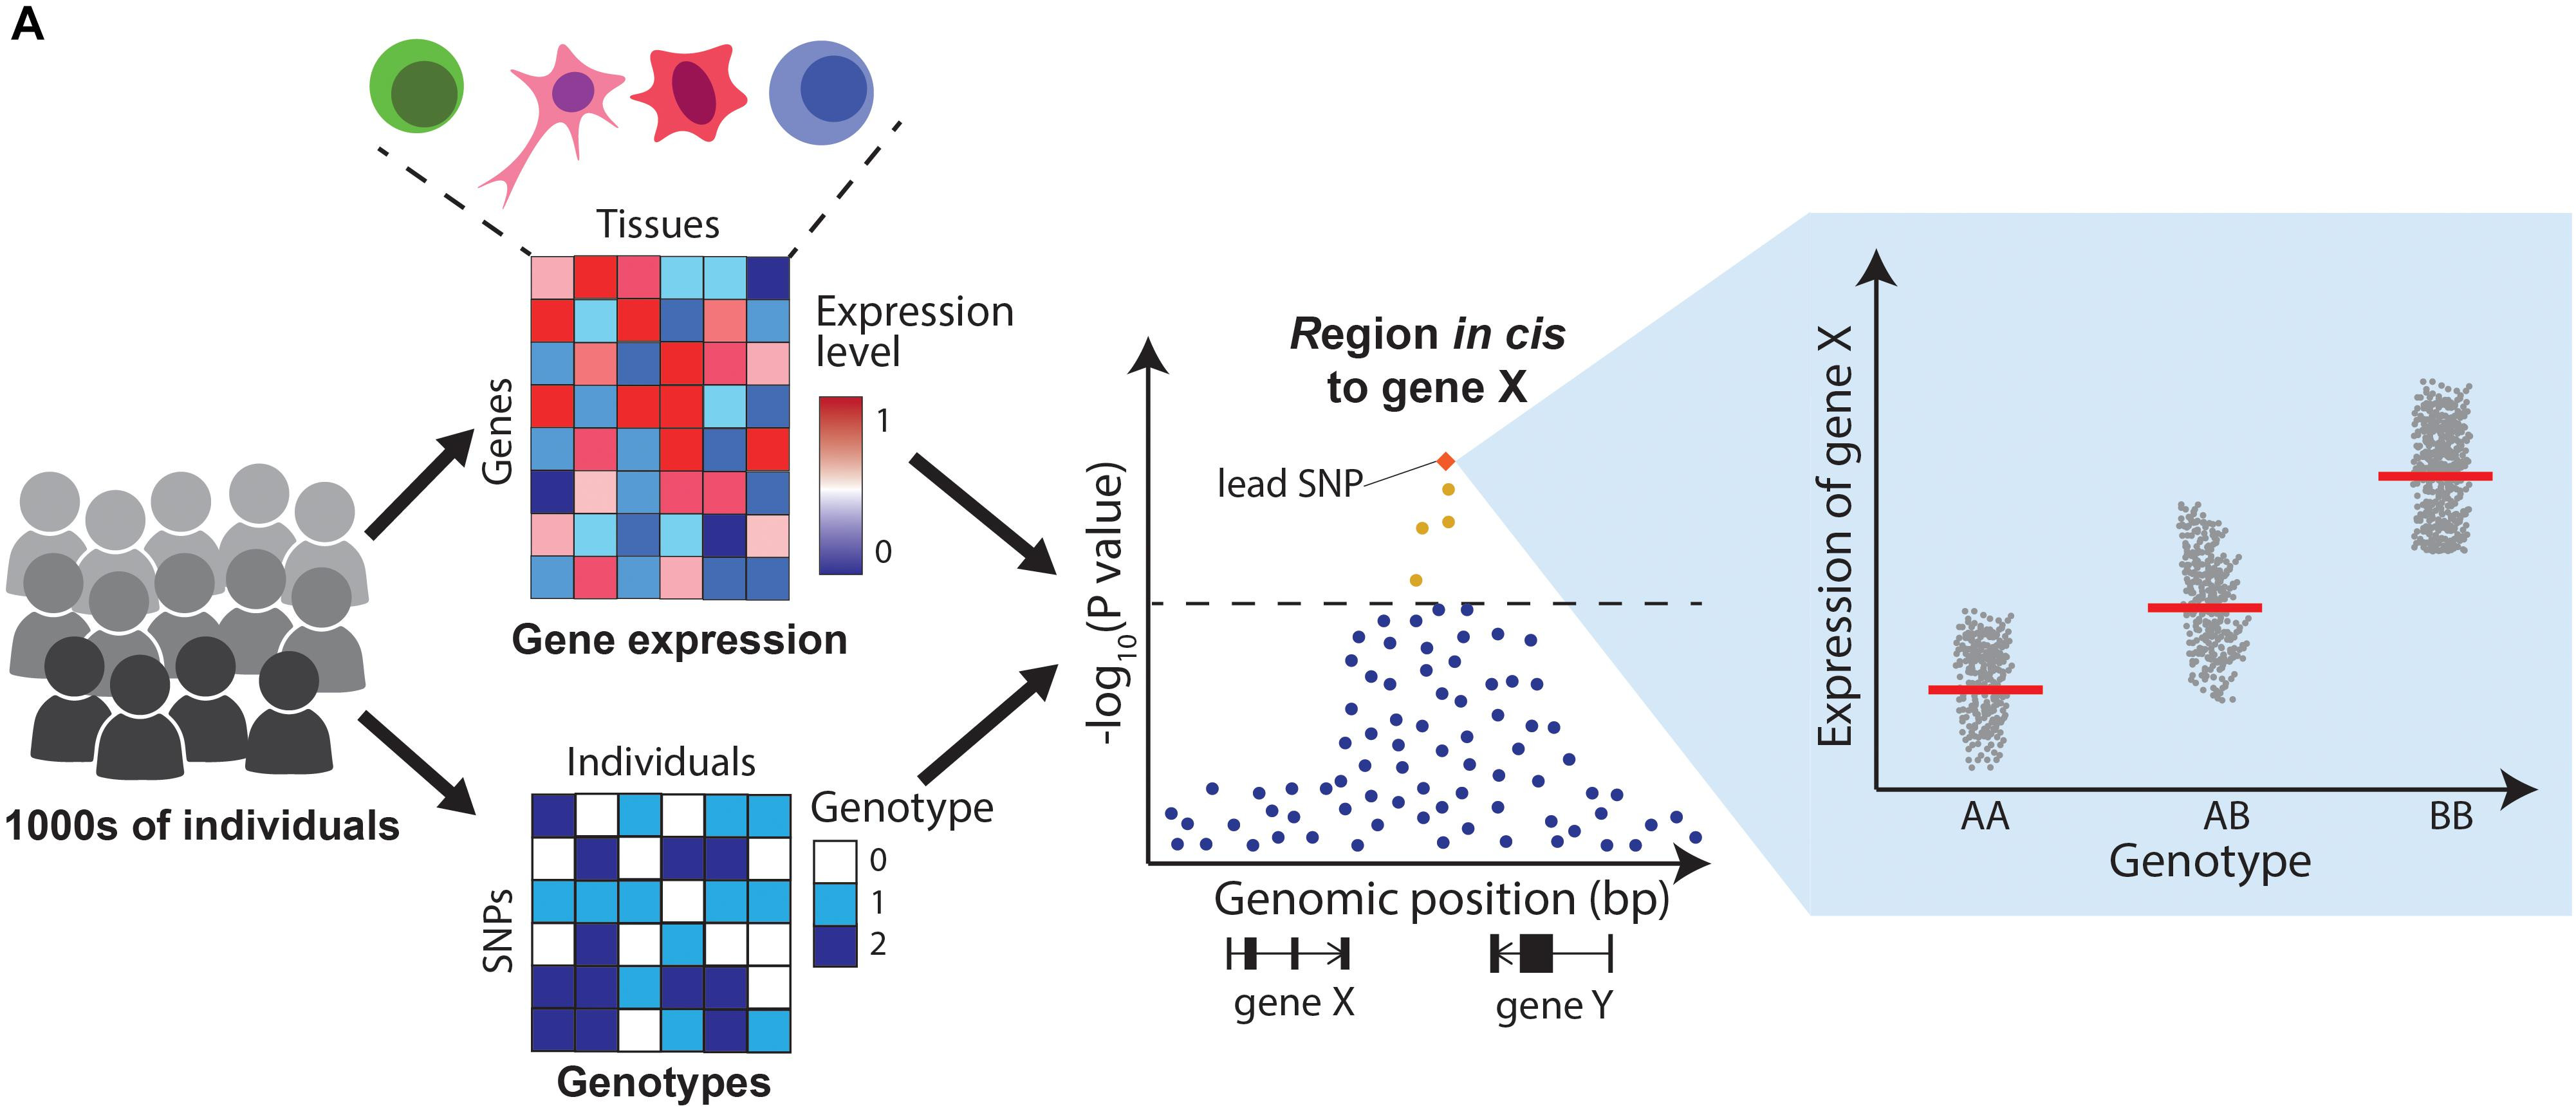
\includegraphics[width=\textwidth]{\presentationgoldparispath/doi_10.3389_fgene.2020.00424_fig4a.jpg}

\let\thefootnote\relax\footnotetext{Cano-Gamez et al. 2020. doi:10.3389/fgene.2020.00424}
\end{frame}

%%%%%%%%%%%%%%%%%%%%%%%%%%%%%%%%%%%%%%%%%%%%%%%%%%%%%%%%%%%%%%%%%%%%%%%%%%%%%%%%
\begin{frame}
\frametitle{Summary}

\begin{center}
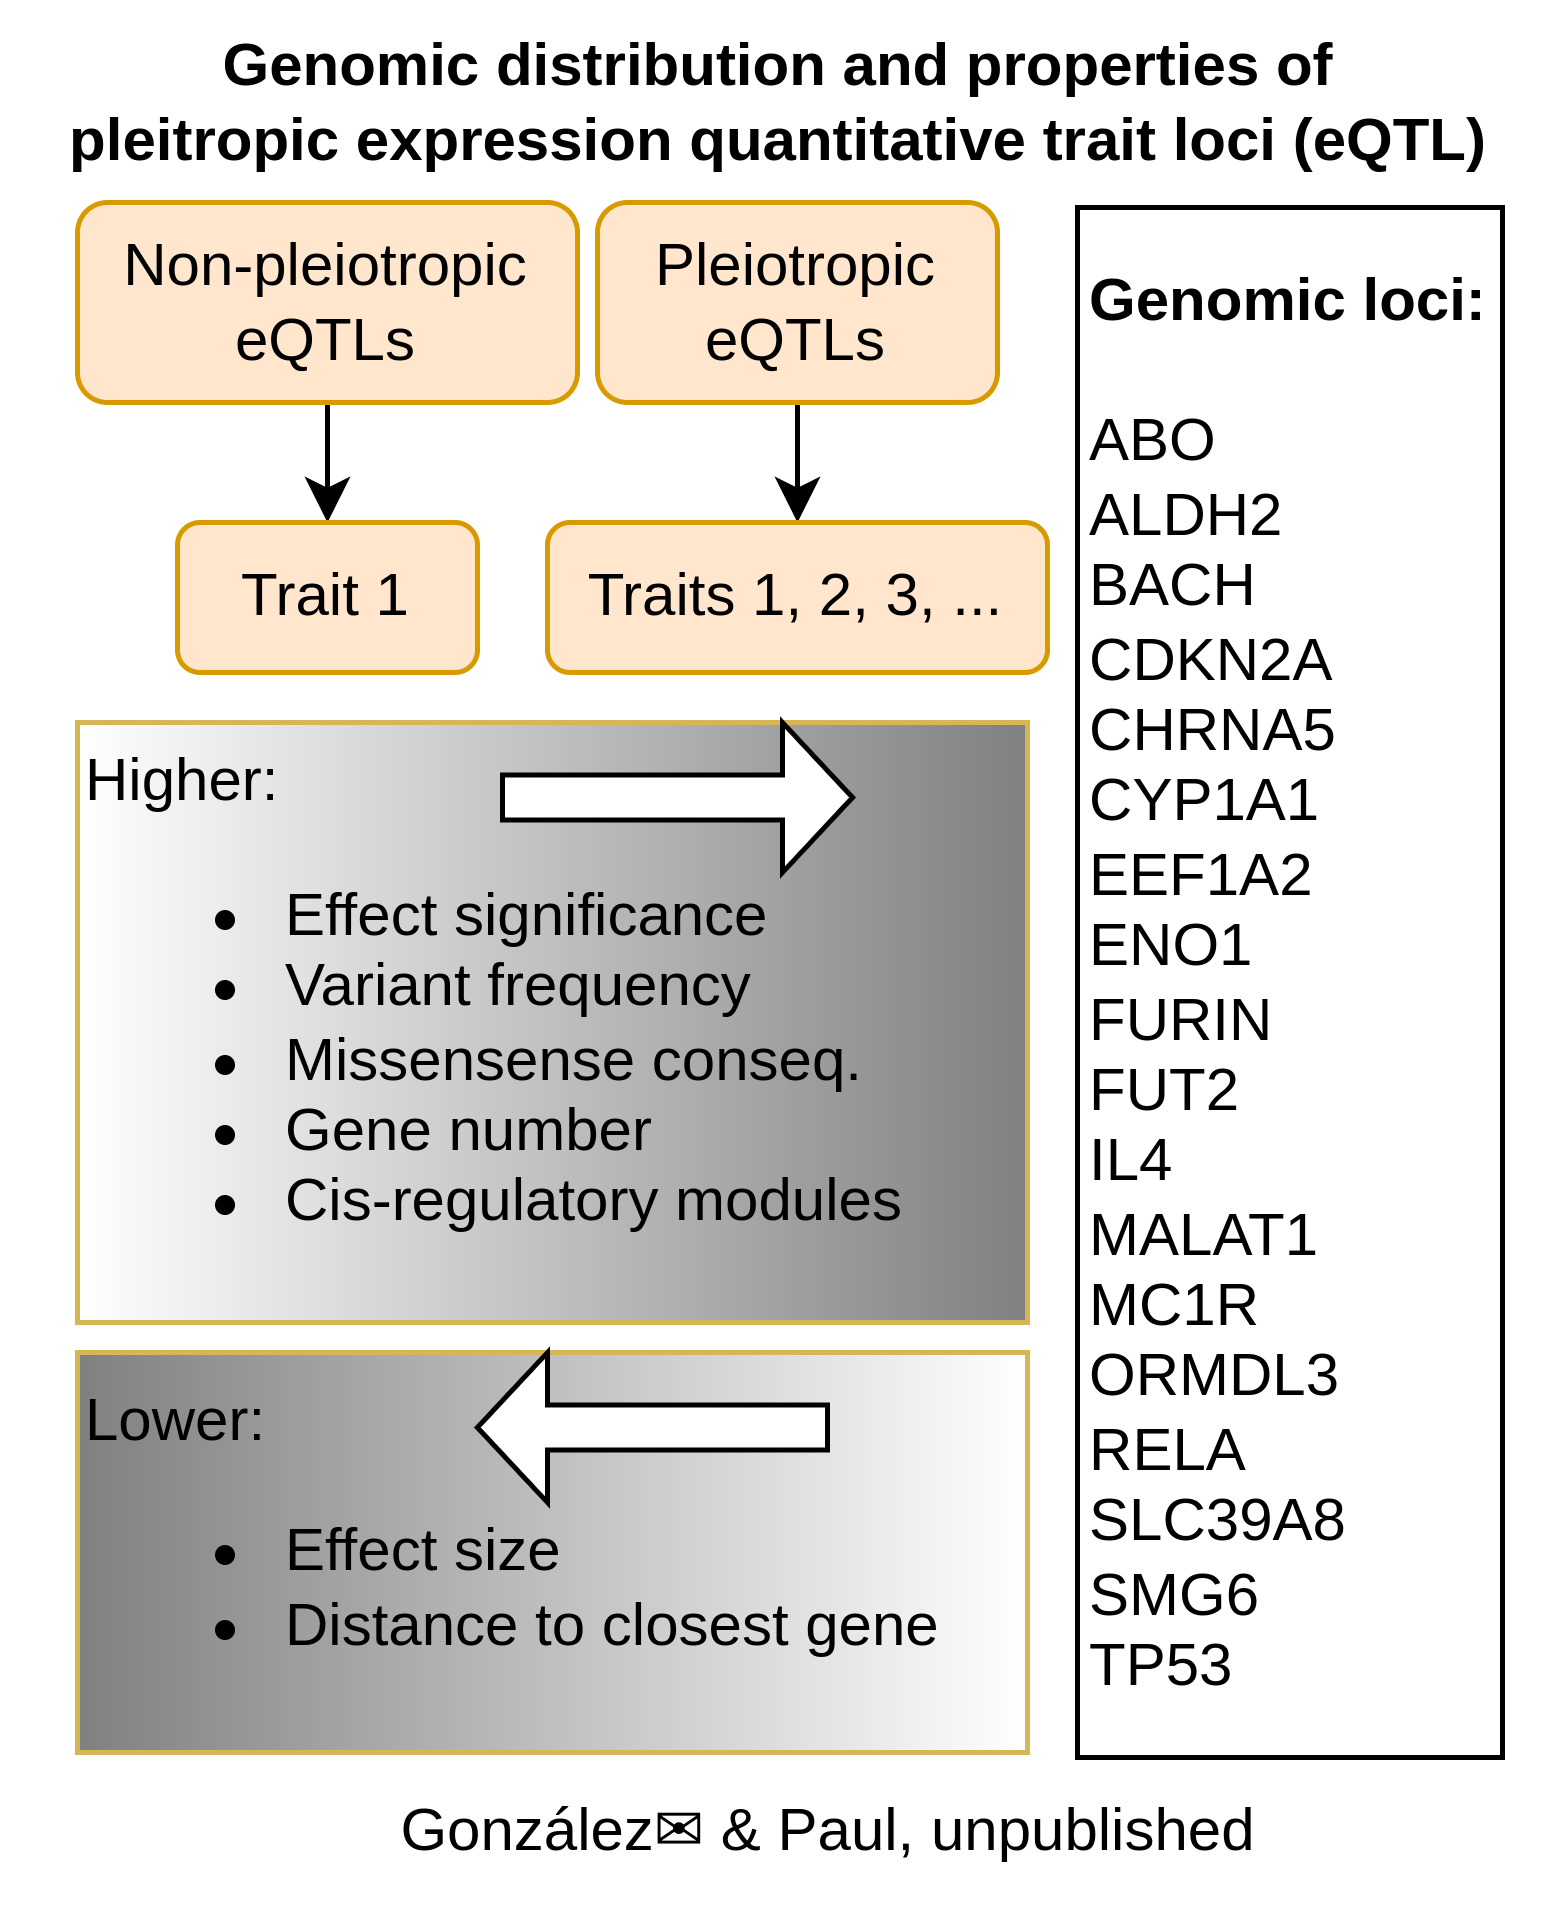
\includegraphics[width=0.5\textwidth]{fig/graphical_abstract.drawio.png}
\end{center}

\end{frame}

\end{document}
